\section{Parte A}
    \subsection{Circuito utilizado}
        \begin{figure} [H] 
            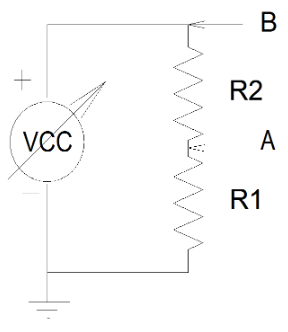
\includegraphics[width=7.5cm]{A-circ}
            \caption{Circuito Utilizado na parte A}
            \label{fig:A-circ}
        \end{figure}
    \subsection{Gráficos}
        \begin{figure} [H] 
            \begin{subfigure}[b]{7cm}  
                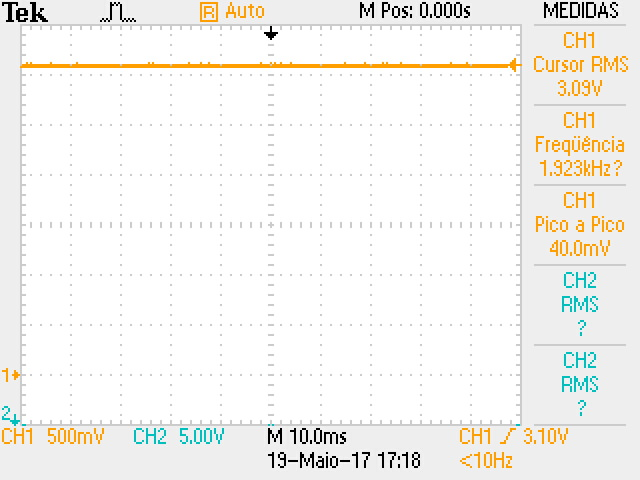
\includegraphics[width=7cm]{A-a-b}
                \caption{Nos pontos A e B}
                \label{fig:A-a-b}
            \end{subfigure}
            \begin{subfigure}[b]{7cm}  
                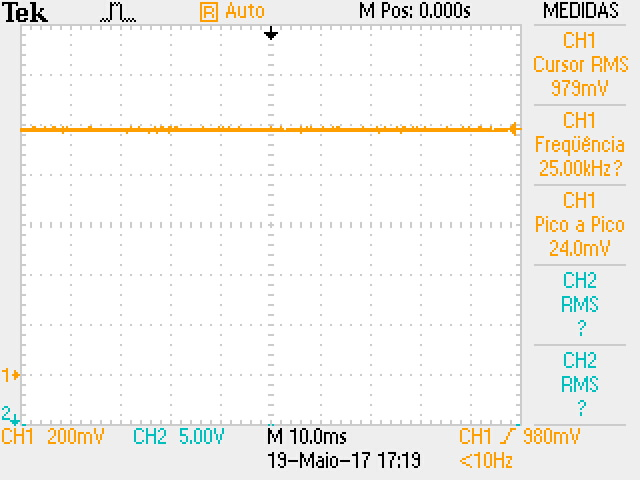
\includegraphics[width=7cm]{A-a-c}
                \caption{Nos pontos A e C}
                \label{fig:A-a-c}
            \end{subfigure}
            \caption{Gráfic Uxt no oscilador na parte A}
        \end{figure}
    \subsection{A3}
        \paragraph{Utilizando a função `Medida`} encontramos 
        $$V_a = (0,98 \pm 0,05) V$$
        $$V_b = (3,1 \pm 0,1) V$$

        Sendo as incertezas encontradas a partir da função de precisão do osciloscópio dada pelo `Série TBS1000 Osciloscópios de Armazenamento Digital ZZZ Manual do Usuário`:
        $$\pm(3\% de |leitura| + 0,05 div + 1mV)$$
        para a configuração de média do osciloscópio. 
        \newline
        
        Logo:
        $$\Delta V_a = \pm(3\% de |leitura| + 0,1 div + 0,001) V = (0,03*0,979 + 0,1*0,2 + 0,001) V \approx 0,05 V$$
        $$\Delta V_b = \pm(3\% de |leitura| + 0,1 div + 0,001) V = (0,03*3,09 + 0,1*0,5 + 0,001) V \approx 0,1 V$$
    \subsection{A4}
        \paragraph{Utilizando o multímetro} encontramos 
        $$V_a = (0,971 \pm 0,005) V$$
        $$V_b = (3,05 \pm  0,01) V$$
        
        Sendo as incertezas encontradas a partir 
        da fórmula de precisão do multímetro dada 
        pelo “Manual de instruções do multímetro 
        digital de bancada modelo MD-6680”: 
        $$\pm(0,3\% * |valor medido| + 2d)$$
        para a configuração de 6 volts em 
        corrente contínua (DC) e precisão de 
        $0,001 V$.
        \newline
        
        Logo: 
        $$\Delta V_a = \pm(0,3\% * |valor medido| + 2d) V = \pm(0,003*0,971 + 0,002) \approx 0,005 V$$
        $$\Delta V_b = \pm(0,3\% * |valor medido| + 2d) V = \pm(0,003*3,053 + 0,002) \approx 0,01 V$$

        Comparando os valores e incertezas das 
        tensões medidas no ponto A e no ponto B 
        pelo osciloscópio e pelo multímetro, 
        vimos que seus valores coincidem. 
        Mesmo que os valores sejam diferentes, 
        suas incertezas possuem pontos em comum, 
        mostrando que os valores medidos pelo 
        osciloscópio e pelo multímetro sejam 
        praticamente o mesmo.